\documentclass[10pt,twocolumn,letterpaper]{article}

\usepackage{cvpr}
\usepackage{times}
\usepackage{epsfig}
\usepackage{graphicx}
\usepackage{amsmath}
\usepackage{amssymb}

\usepackage{enumitem}
\usepackage{url}

% Include other packages here, before hyperref.

% If you comment hyperref and then uncomment it, you should delete
% egpaper.aux before re-running latex.  (Or just hit 'q' on the first latex
% run, let it finish, and you should be clear).
\usepackage[breaklinks=true,bookmarks=false]{hyperref}

\cvprfinalcopy % *** Uncomment this line for the final submission

\def\cvprPaperID{****} % *** Enter the CVPR Paper ID here
\def\httilde{\mbox{\tt\raisebox{-.5ex}{\symbol{126}}}}

% Pages are numbered in submission mode, and unnumbered in camera-ready
%\ifcvprfinal\pagestyle{empty}\fi
\setcounter{page}{4321}
\begin{document}

%%%%%%%%% TITLE
\title{All Convolutional Net for Recognition and Transfer Learning Tasks}

\author{Shuailin Li\\
ShanghaiTech University\\
% lishl@shanghaitech.edu.cn\\
{\tt\small lishl@shanghaitech.edu.cn}
% For a paper whose authors are all at the same institution,
% omit the following lines up until the closing ``}''.
% Additional authors and addresses can be added with ``\and'',
% just like the second author.
% To save space, use either the email address or home page, not both
\and
% Second Author\\
% Institution2\\
% First line of institution2 address\\
% {\tt\small secondauthor@i2.org}
}

\maketitle
%\thispagestyle{empty}

%%%%%%%%% ABSTRACT
\begin{abstract}
   Striving for simplicity, the all convolutional net is proposed by Jost
    in \cite{striving}. Followed by his baseline, we implement the same networks to verify
     his conclusions. We find it true that pooling layers can be replaced by 
     convolution layers with stride. On the other hand, with the same network, 
     we design a transfer learning experiment, indicating that transfer learning 
     outperforms the strategy that trains from scratch, especially for small datasets.
\end{abstract}

%%%%%%%%% BODY TEXT
\section{Introduction}
Alternating convolution and max-pooling layers are a trend to design forehead of convolutional neural networks(CNN). However, Jost proposed that pooling layers are not a must for object recognition network in \cite{striving}. His work attempts to search for a simple recognition network and build a baseline on common datasets. In this work, we follow his baseline, to verify the role of pooling layers, and design experiments on transfer learning. Though we still cannot reach the state of the art in his work, the conclusions are the same: “max-pooling can simply be replaced by a convolutional layer with stride”. On the other hand, transfer learning approach is of great importance for recognition on small dataset.

\section{Model Review}
There are 6 models are implemented in our experiment, corresponding to model A, B, C, Strided-CNN-C, ConvPool-CNN-C and All-CNN-C in \cite{striving} separately.

Three base networks are named as ANet, BNet and CNet. High level layers of three models are the same, while foreheads are distinct. Three models are designed to check optimal options of kernel size and stacked conv layers. To be specific, they are all a sequential net alternating conv layers and pool layers, and differences fall on the kernel size of conv layers. The optional kernel sizes are 5x5, 1x1 and 3x3.

Based on CNet, three variations are derived, for evaluating the importance of pooling. They are model Strided-CNN-C, ConvPool-CNN-C and All-CNN-C,  short as SCC, CCC, ACC. To achieve the target evaluation, the max-pooling layer is removed and the stride of the precious layer is increased in SCC and ACC. On the other hand, an additional convolution layer is applied in CCC and ACC, in order to prove that deep layers outperform shallow layers.

Our experiments are on Mac OS X, with Pytorch 1.0 and Python version 3.6.The implementation on Pytorch is based on many materials. \cite{style} offer a fine-structured code organization, \cite{torch} provides transfer learning examples, and a routine of training procedure is from \cite{acc}.

We experiment on two dataset, CIFAR-10 and CIFAR-100. All six models are used in CIFAR-10 to check the importance of pool layers and deep networks. While only ACC(ALL-CNN-C) used in CIFAR-100, to do transfer learning experiment. More details about datasets and objectives are in later part.

\section{Experiment}
    \subsection{Dataset}
    The CIFAR-10 dataset consists of 60000 32x32 colour images in 10 classes, with 6000 images per class. There are 50000 training images and 10000 test images. In our experiment, all networks are trained using stochastic gradient descent with fixed momentum of 0.9. The learning rate lr is select from the series {1e-1, 1e-2, 1e-3, 1e-4}, and finally fix it as lr = 1e-2, which leads to best performance. According to convergence curve of training accuracy, we set lr\_scheduler as CosineAnnealingLR in pytorch, and T\_max as 50. Different from suggestive epoch value, we find it sufficient to set epoch as 100 rather than 350. By contrast experiment, it is useless to use dropout regularizer here, thus we discard it. Additionally, all models are regularized with weight decay 0.0001. As for data augmentations, we only use random crop, horizontal flip and normalize operations, while randomly translated versions, whitened and contrast normalized images are used in \cite{striving}. 
    
    In particular, it is necessary to do weight initialization. In practice, the training went to a failure without initialization. At the moment, we use Xavier Initialization to initialize all conv layers.

    
    Two subsets of CIFAR-100 are picked up for transfer learning experiments. The subsets are class1 and class2, each contains 10 classes and is divided into training set of 5000 and test set of 1000. For class1, it has similar categories as previous CIFAR-10, while much different categories are contained in class2. This setting is interesting, we are convinced intuitively that model pretrained on CIFAR-10 is able to achieve good performance on class1, but how about class2? In other word, we are to examine the generalization of stacked layers in low level as a feature extractor.

    \subsection{Results}

        % table 1
        \begin{table}[]
            \begin{tabular}{lcc}
            \hline
            Model & Accuracy (\%) & SOTA (\%) \\
            \hline
            ANet  & 85.33         & 87.53     \\
            BNet  & 86.84         & 89.80     \\
            CNet  & 88.74         & 90.26     \\
            SCC   & 88.86         & 89.81     \\
            CCC   & 89.42         & 90.69     \\
            ACC   & 89.21         & 90.92     \\
            \hline
            \end{tabular}
            \caption{Comparison of test accuracy between our results and the state of the art on the CIFAR-10 dataset.}
            \label{tab: t1}
            \end{table}
            
            
            % table 2
            \begin{table}[]
            \begin{tabular}{llc}
            \hline
            Dataset & Training Strategy & Accuracy (\%) \\
            \hline
            class 1 & transfer learning & 83.6          \\
            class 1 & from scratch      & 73.3          \\
            class 2 & transfer learning & 84.5          \\
            class 2 & from scratch      & 73.5          \\
            \hline
            \end{tabular}
            \caption{Comparison between transfer learning and from scratch strategy on the CIFAR-100 dataset.}
            \label{tab: t2}
            \end{table}


    The results of all models are given in Table \ref{tab: t1} and Table \ref{tab: t2}  , and the results of \cite{striving} are presented as a comparison. Several points are verified in our results from the table. We discuss the first 6 model in this paragraph, ignoring transfer learning temporarily. First, for three base networks, model C outperforms model A and model B, it is mainly because large receptive fields of stacked 3x3 convolution layers. Though with slight increasement of  parameters, the last architecture is superior to classification tasks. Second, ’Strided-CNN-C’ perform competitively with  model C and so as ‘All-CNN-C’ versus ‘ConvPool-CNN-C’, which suggests that max-pooling layer can be replaced by a convolution layer with stride r=2 — the same conclusion as \cite{striving}. Thirdly, according to the performance of ’89.21%’ vs. ’88.86%’, deeper network is better. 
    
    The results of our work is inferior to the work in \cite{striving}, some tricks may contribute to this gap. The first is the parameter ‘epoch’ and ‘dropout’ operation, in our work, we use epoch=100 without dropout, which is much smaller than proposed epoch=350, due to time constraint. Secondly, aggressive data augmentation in \cite{striving} increase the ability of generalization extensively, while we only use several augmentation operations(random crop, horizontal flip and normalize operations). Additionally, there are some details we have not paid attention to.

    Next, it is time to discuss the results of transfer learning. From the table, the networks with transfer learning strategy outperform ones with from-scratch strategy. Comparisons indicates the efficiency and effectiveness of transfer learning, especially considering that ones with transfer learning converge faster. Due to pretrained feature extractor of ACC network, the performance differences are interpretable, and verifying the importance of transfer learning. 
    
    It is worthy noting that datasets of class1 and class2 comprise 10 similar categories and 10 distinct categories separately, in view of result curves, they converge in competitive speed and reach a similar accuracy finally. It evince us that low level layers as the feature extractor is indifferent to concrete classes. Considering the fact that size of the training data is 5000 and the size of previous data is 50000, transfer learning can provide more priori than of from scratch. In a sense, when lacking of training data, transfer learning bring information of other data, and push the inference level to a amazing height. 

        % figure 1
        \begin{figure}
            \centering            
            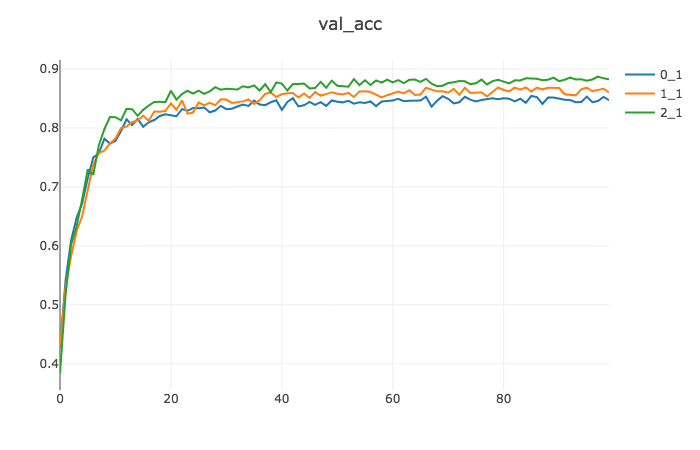
\includegraphics[width=\linewidth]{seolen_fig/BaseNet_VA.png}
            \caption{Accuracy curves of base models on CIFAR-10. 0, 1, 2 correspond to model A, B, C.}
            \label{fig:a}
        \end{figure}

        % figure 2
        \begin{figure}
            \centering            
            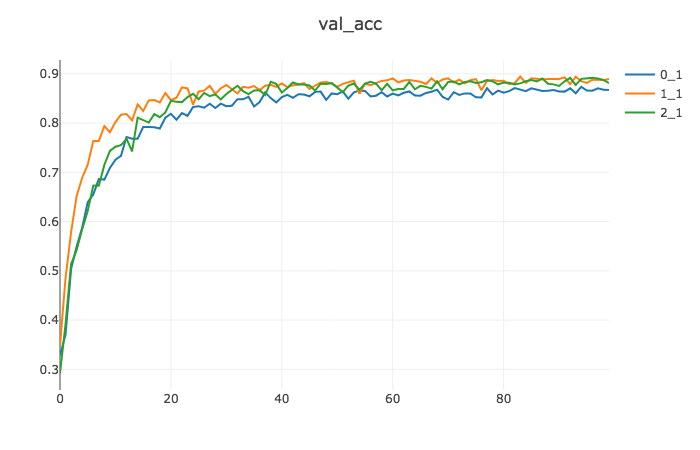
\includegraphics[width=\linewidth]{seolen_fig/VNET_3_VA.png}
            \caption{Accuracy curves of variation models on CIFAR-10. 0, 1, 2 correspond to model Strided-CNN-C, ConvPool-CNN-A, All-CNN-C.}
            \label{fig:b}
        \end{figure}

        % figure 3
        \begin{figure}
            \centering            
            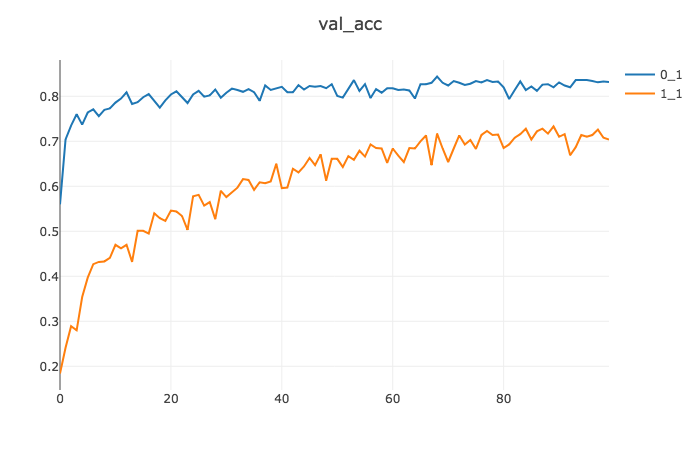
\includegraphics[width=\linewidth]{seolen_fig/Transfer_class1_VA.png}
            \caption{Accuracy curves of  All-CNN-C models on class 1 of CIFAR-100. 0, 1 correspond to transfer learning and from scratch.}
            \label{fig:c}
        \end{figure}

        % figure 4
        \begin{figure}
            \centering            
            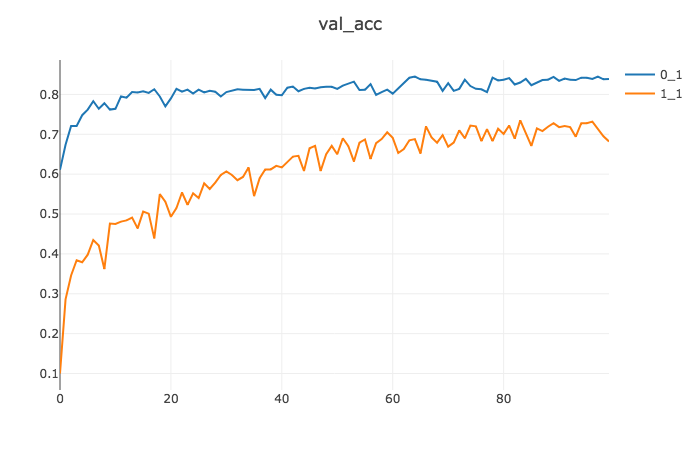
\includegraphics[width=\linewidth]{seolen_fig/Transfer_class2_VA.png}
            \caption{Accuracy curves of  All-CNN-C models on class 2 of CIFAR-100. 0, 1 correspond to transfer learning and from scratch.}
            \label{fig:d}
        \end{figure}

\section{Conclusion}
To conclude, we highlight a few key observations that we made in our experiment:
    \begin{enumerate}
        \item We verify the observation that a network with only convolutions and subsampling matches the state of the art on CIFAR-10. At least on this scale of classification task, max-pooling is not a must.
        \item A deep network outperform a shallow one, at the same time, the gap of results with and without max-pooling is narrowed in deep network.
        \item Transfer learning brings high convergence speed and high accuracy, and superior than training from scratch in a small dataset.
    \end{enumerate}









{\small
\bibliographystyle{ieee}
\bibliography{egbib}
}

\end{document}
